\chapter{Design, Simulation and Verification Tool}
\label{chap:simulation}

This chapter describes a design, simulation and verification software tool
developed by the author during the research period. In order to show the
motivation underlined the tool development a breve observation of existing
publicly accessible tools is presented, as well as requirements for such
software. Then an application of the tool is demonstrated on the
example of industrial plant, which is described in the Chapter
\ref{chap:problem_description}.


\section{Requirements for Formal Tools}

According to the survey, that was presented in
\cite{blackburn_requirements_1998}, the industrial and research communities,
\emph{there is a need for �light-weight� formal methods and associated tools,
where engineers can �push-the-button� and have powerful evaluations and analysis
take place}. More than one decade later, this need has been even grown, and
requirements the authors imposed are still actual. Shortly, the requirements are:
\begin{itemize}
  \item Formal methods should be ``invisible'' and automatic
  \item Usage of open standards for sharing formal results
  \item Easy to use (either in academic or industrial field)
  \item Modular structure, lightweight architecture
  \item Scalable for real world problems
\end{itemize}

Nowadays, numerous commercial software tools can be found on market and even
more accessible with no charge. Verilog hardware description language
\cite{verilog}, Event-B and Roding \cite{event_b_web}, ProB model checker
\cite{theprob}, Pessoa \cite{pessoa} to mention a few. These tools aimed for  
complex task and are capable to solve heave industrial-like problems. The
lightweight academical response is GOAL \cite{goal}, DESUMA \cite{desuma},
TCT \cite{tct}, Supremica \cite{supremica}, etc.

Some of the tools are of high quality, other are easier to use. But the major
drawback of the aforementioned software is that it is closed for modification,
which makes it is almost impossible to use it for a research, for creation and
validation of new formal techniques. An appropriate software tool for the
studying and research purpose is desired to be easy to access, working on most
of hardware and software platforms, flexible for changes, and with an intuitive
user interface design.

Bearing in mind the above motivation, a specialised software tool was created in
frame of this work. Its primary goal was a validation of concepts developed
during the research. It provides simple access and zero-time enrollment time on
general operational systems due to the exploiting web-technologies. It was
thought as a Free Open Source Software (FOSS) tool with potential of enhancement
by a wide community interested in it. 

The main disadvantage of the web-based underlining approach is a relatively low
performance due to the nature of the programming languages used. However, the
last trends in web development show that this issue can be overcome in a near
future.

\section{Tool Description}

The charasterics of software tool developed during the research project are
summarised in the Table \ref{tbl:tool_commands}. The objects and operations
allow to cover many tasks while formal techniques development. Additional
methods can be easily implemented. 

As a programming language a general purpose web-oriented language was chosen,
the JavaScript. For the sake of memory efficiency, a set--based approach was
chosen for automata structural representation (see \ref{soft_methods_2005} for
the approaches). The current graphical implementation exploits  Scalable
Vector Graphics (SVG) \cite{web_svg}. This allows use of any graphical
representation (e.g. automata, influence diagrams) to be used with no
translation in the most of types of documents. An instance of the screen of the
tool is shown in the Figure \ref{fig:editor_screen}.


\begin{table}[!ht]
\caption{Objects and operations available with the tool}
\centering
	\begin{tabular}{l l }
	\\	
	Object & Operations\\
	\hline
	Sets & Binary, Numbers, Strings and Objects operations \\
	Sets & Operations on triples (for graph edges/transitions) \\
	Graph & Manipulations with edges and nodes \\
	Graph & Breadth-First Search (BFS) in a graph \\
	Graph & Depth-First Search (DFS) in a graph \\
	Graph & Automatic layout\\
	Automata & Parallel composition of two automata \\
	Automata & Intersection (full synchronisation)\\
	Automata & Kleene closure \\
	Automata & Subtraction \\
	Automata & Emptiness verification \\
	Automata & Copying operation \\
	Automata & Projection to a given set of events \\
	Automata & Complement operation \\
	Automata & Reachability operation \\
	DES & Centralized management of the events set\\
	DES & Creation of a module in frame of the DES\\
	DES & Creation of an external module \\
	DES & Computation of common events of two automata \\
	DES & Representation of the system with as the inference diagram \\
	Diagnosability & Fault states and events support \\ 
	Diagnosability & Computations of automata deterministic w.r.t. a failure
	history\\
	Diagnosability & Computation of fault-reachable and fault-non reachable
	languages\\
	
	\hline
	\end{tabular}
	\label{tbl:tool_commands}
\end{table}


\begin{figure}[!h]
	\centering
	\includegraphics[scale=0.5]{editor_screen.png}
	\caption{View of the simulator in a browser window}
	\label{fig:editor_screen}
\end{figure}


\section{Diagnosability verification of the system}

In this section the problem of diagnosability verification of the system
presented in the Chapter \ref{chap:problem_description} is studied. In order to
validate the theoretical approach and the algorithms introduced in this work a
formal model of the system has to be constructed. The model contains automata
of the component types listed in the Table \ref{tbl:system_modules}.
Moreover, the model contains automata which describe supervisory control
policy for each control cycle. 

\begin{table}[th]
\caption{Modules of the system depicted in the Figure \ref{fig:pi_diagram}}
\centering
	\begin{tabular}{l c}
	\\	
	Module name & Number of modules \\
	\hline
	Butterfly valve	& 2 \\
	Gate valve	& 3 \\
	Screw conveyer	& 1 \\
	Vibrator		& 1 \\
	Belt conveyer	& 1 \\
	Fork level sensor	& 4 \\
	Air pump	& 1 \\
	\hline
	\end{tabular}
	\label{tbl:system_modules}
\end{table}

Automata models of the system's physical components are constructed according to
design patterns of the Generalized Device approach. Types of automata 
and composition techniques used to model this system are presented in
Appendix \ref{chap:automata_models}. 

The resulting inference diagram of the system is depicted in the Figure
\ref{fig:system_id}. The diagram is built automatically by the simulation tool.
It is interesting to see how the nodes which represent the control policy
automata link all the nodes representing filed devices into the whole.

\begin{figure}[!ht]
	\centering
	\includegraphics[scale=0.5]{system_id.pdf}
	\caption{Inference diagram of the system depicted in the Figure
	\ref{fig:pi_diagram}}
	\label{fig:system_id}
\end{figure}


\subsection{Global model of the system} 

Global monolithic model of a system is required for verification of
centralized diagnosability. An attempt to construct the global model of a
real complex system usually faces the states explosion problem. 

The presented system with the current design consists of \emph{53}
automata. Using the simulation tool, an attempt to construct the monolithic
model was made. Table \ref{tbl:sync_growth} shows the growth of the automaton of
the monolithic model by means of states, transitions and time spent for each
iteration.
The corresponding plot is depicted in the Figure \ref{fig:sync_growth}. 

The given system has relatively low complexity. Construction of the global model
using another tool like NuSMV \cite{nusmv} is likely possible. However, the
tool used in this case has performance not optimised yet, and the construction
of the global model was performed only partially due to the time limit.

\begin{table}[!ht]
\caption{Growth of the centralized model during parallel composition}
\centering
	\begin{tabular}{c r r l}
	\\
	Number of modules & States & Transitions & Time spent, min:sec.ms \\
	\hline
	2 & 10 & 46 & 0:0.4 \\
	3 & 20 & 132 & 0:0.37 \\
	4 & 22 & 122 & 0:0.5 \\
	5 & 21 & 96 & 0:0.3 \\
	6 & 63 & 498 & 0:0.12 \\
	7 & 63 & 460 & 0:0.10 \\
	8 & 63 & 424 & 0:0.11 \\
	9 & 315 & 2939 & 0:0.78 \\
	10 & 630 & 7138 & 0:0.406 \\
	11 & 1260 & 16796 & 0:1.627 \\
	12 & 1386 & 17014 & 0:1.686 \\
	13 & 1323 & 14952 & 0:1.282 \\
	14 & 3969 & 58086 & 0:7.701 \\
	15 & 3969 & 55692 & 0:8.579 \\
	16 & 3969 & 53424 & 0:7.866 \\
	17 & 19845 & 318717 & 3:43.389 \\ 	
	18 & 39690 & 716814 & 23:41.914 \\ 
	\hline
	\end{tabular}
	\label{tbl:sync_growth}
\end{table}

\begin{figure}[!ht]
\centering
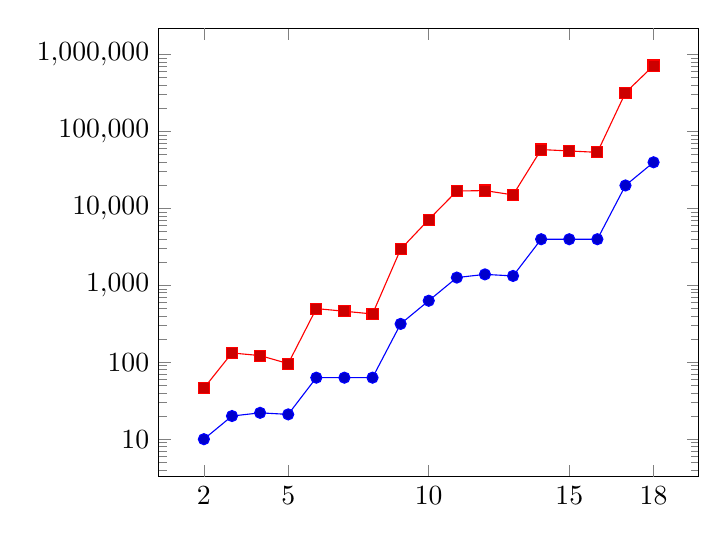
\begin{tikzpicture}
\begin{axis}[
    ymode=log,
    log ticks with fixed point,
    extra x ticks={2,18}
]
\addplot table {
	2 10
	3 20
	4 22
	5 21
	6 63
	7 63
	8 63
	9 315
	10 630
	11 1260
	12 1386
	13 1323
	14 3969
	15 3969
	16 3969
	17 19845
	18 39690 
};
\addplot table {
	2 46
	3 132
	4 122
	5 96
	6 498
	7 460
	8 424
	9 2939
	10 7138
	11 16796
	12 17014
	13 14952
	14 58086
	15 55692
	16 53424
	17 318717 	
	18 716814 
};
\end{axis}
\end{tikzpicture}
	\caption{Growth of the number of states (curve with round dots) and
	transitions (curve with square dots) while the growth of the number of modules
	in the centralized systems model}
	\label{fig:sync_growth}
\end{figure}


\subsection{Example of a failure verification}

For a demonstration of diagnosability verification with the developed tool
the instance of a hypothetical technological failure is taken (though it could
be a real case for the given system). A part of the material flow
description, given by a technologist is following.

Consider the P\&I diagram of the system  depicted in the Figure
\ref{fig:pi_diagram}. Volumes of the filter container and of the dust bucket are
chosen according to a speed the filter container fills up, the dust bucket
unloads and a speed of the material transportation by the both screw and
belt conveyers. When the filter container is filled, it takes two times to
load and unload the dust bucket. Due to physical limits of the process, the
filter conveyer can not be emptied with one load--unload cycle of the dust
bucket, neither the filter container can be full after two unload cycles.
An automaton model which may describe this technological process is depicted in
the Figure \ref{fig:system_failure02}.

The automaton reflects also possible failures (shown with the marked state of
the automaton).
If the filter container is empty just after one unload, this may be a symptom of the screw conveyer breakage,
destruction of the pipe or its connection to the valve. If the filter container
is full after three unload cycles, it may be a sign of low dust bucket
performance, pipes clogging, etc.

\begin{figure}[!ht]
	\centering
	\includegraphics[scale=0.7]{system_failure02.pdf}
	\caption{Model of a technological process failure}
	\label{fig:system_failure02}
\end{figure}

The failure automata model does not contain any observable events. Thus, the
model is not diagnosable locally. However, the model can be linked to the fork
level sensors $LT1$ and $LT3$ as with digital signals via cause-effect automata
(see description in the Appendix \ref{chap:automata_models}).

The diagnosability of the system was verified using the tool presented earlier.
The forward-propagation algorithm performed 356 compositions of the modules in
less then a second. During the failure propagation through the inference diagram
(see Figure \ref{fig:system_id}) six modules where updated while a little
complexity growth was observed. The verification has shown that in the diagnosis
of the failure two modules of the system participate, the sensors $LT1$ and
$LT3$. According to the approach of this work, these modules can be treated as
one virtual module. This virtual module can be used to build diagnoser for
online monitoring of the system, particularly for detection of the above
described failure.



